\begin{figure}[htbp]
\centering
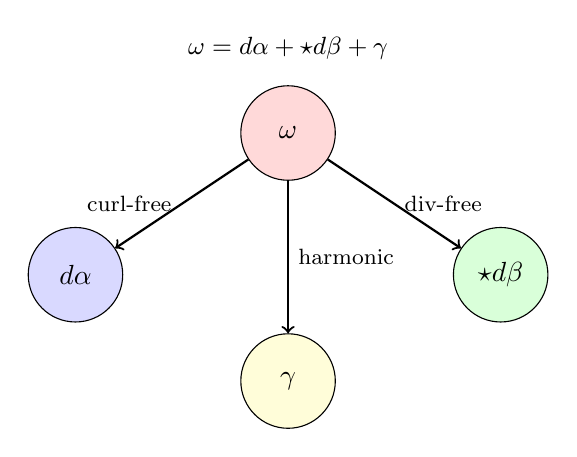
\begin{tikzpicture}[scale=0.9]
  \node[draw,circle,fill=red!15,minimum size=1.2cm] (omega) at (0,0) {$\omega$};
  \node[draw,circle,fill=blue!15,minimum size=1.2cm] (exact) at (-3,-2) {$d\alpha$};
  \node[draw,circle,fill=green!15,minimum size=1.2cm] (coexact) at (3,-2) {$\star d\beta$};
  \node[draw,circle,fill=yellow!15,minimum size=1.2cm] (harmonic) at (0,-3.5) {$\gamma$};
  \draw[->,thick] (omega)--(exact) node[midway,left,font=\footnotesize] {curl-free};
  \draw[->,thick] (omega)--(coexact) node[midway,right,font=\footnotesize] {div-free};
  \draw[->,thick] (omega)--(harmonic) node[midway,right,font=\footnotesize] {harmonic};
  \node[font=\small,align=center] at (0,1.2) {$\omega = d\alpha + \star d\beta + \gamma$};
\end{tikzpicture}
\caption{Hodge decomposition: any 1-form $\omega$ splits uniquely into exact, co-exact, and harmonic components.}
\label{fig:hodge_decomp}
\end{figure}
